% !TEX root = ./main.tex

\section{Qualitative and semiquantitative checks that can rule out good sampling}
\label{sec:quick}

It is difficult to establish with certainty that good sampling has been achieved, but it is not difficult to \emph{rule out} high-quality sampling.
Here we elaborate on some relatively simple tests that can quickly bring out inadequacies in sampling.

Generally speaking, analysis routines that extract information from raw simulated data are often formulated on the basis of physical intuition about how that data should behave.  Before proceeding to quantitative data analysis and uncertainty quantification, it is therefore useful to assess the extent to which data conforms to these expectations and the requirements imposed by either the modeler or the analysis routines.  Such tasks help reduce subjectivity of predictions and offer insight into when a simulation protocol should be revisited to better understand its meaningfulness \cite{patrone1}.  Unfortunately, general recipes for assessing data quality are impossible to formulate, owing to the range of physical quantities of interest to modelers.  Nonetheless, several example procedures will help clarify the matter.

\subsection{Zeroth-order system-wide tests}
\label{sec:zeroth}

The simplest test for poor sampling is lack of equilibration: if the system is still noticeably relaxing from its starting conformation, statistical sampling has not even begun, and thus by definition is poor.  As a result, the very first test should be to verify that the basic equilibration has occurred.  To check for this, one should inspect the time series for a number of simple scalar values, such as potential energy, system size (and area, if you are simulating a membrane or other system where one dimension is distinct from the others), temperature (if you are simulating in the NVE ensemble), and/or density (if simulating in the isothermal-isobaric ensemble).

Simple visual inspection is often sufficient to determine that the simulation is systematically changing, although more sophisticated methods have been proposed (see Sec.\ \ref{sec:equil}).  If \emph{any} value appears to be systematically changing, %then the system is not equilibrated.
then the system may not be equilibrated and further investigation is warranted.
See, for example, the time trace in Fig.\ \ref{f:rmsd}.
After the rapid rise, the value shows slower changes;
however, it does not fluctuate repeatedly about an average value, implying it has not been well-sampled.


\subsection{Tests based on configurational distance measures (e.g., RMSD)}
\label{sec:bio_RMSD}

\begin{figure}
  \centering
  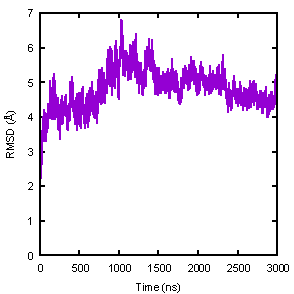
\includegraphics[width=0.9\linewidth]{figures/rmsd}
  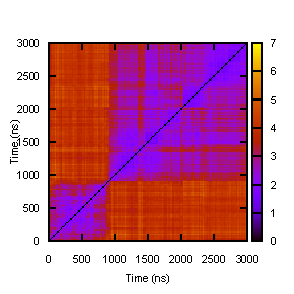
\includegraphics[width=0.9\linewidth]{figures/rmsds}
  \caption{RMSD as a measure of convergence.  The upper panel shows the
    $\alpha$-carbon RMSD of the protein rhodopsin from its starting structure as a
    function of time.  The lower panel shows the all-to-all RMSD map computed from the same
    trajectory.  Color scale is the RMSD, in {\AA}.  Data from Ref.\ \cite{Grossfield-2015}.}
  \label{f:rmsd}
\end{figure}


Because a system with $N$ particles has a $3N$ dimensional configuration-space (the full set of $x, y, z$ coordinates), it is generally difficult to assess the extent to which the simulation has adequately explored these degrees-of-freedom.  Thus, modelers often project out all but a few degrees of freedom, e.g., monitoring a ``distance'' in configuration space as described below or keeping track of only certain dihedral angles.  In this lower dimensional subspace, it can be easier to track transitions between states and monitor similarity between configurations.  However, the interpretation of such analyses requires care.

By employing a configuration-space ``distance'', several useful qualitative checks can be performed.
Such a distance is commonly employed in biomolecular simulations (e.g., RMSD, defined below) but analogous measures could be employed for other types of systems.
A configuration-space distance is a simple scalar function quantifying the similarity between two molecular configurations and can be used in a variety of ways to probe sampling.

To understand the basic idea behind using a distance to assess sampling, consider first a one-dimensional system, as sketched in Fig.\ 1.  If we perform a simulation and monitor the $x$ coordinate alone, without knowing anything about the landscape, we can get an idea of the sampling performed simply by monitoring $x$ as a function of time.  If we see numerous transitions among apparent metastable regions (where the $x$ values fluctuates rapidly about a local mean), we can conclude that sampling likely was adequate \emph{for the configuration space seen in the simulation.}  An important caveat is that we know nothing about states that were never visited.  On the other hand, if the time trace of $x$ changes primarily in just one direction or exhibits few transitions among apparent metastable regions, we can conclude that sampling was poor -- again without knowledge of the energy landscape.

The same basic procedures (and more) can be followed once we precisely define a configurational distance between two configurations.  A typical example is the root-mean-square deviation,
\begin{equation}
\label{eq:rmsd}
\mathrm{RMSD}(\mathbf{r}, \mathbf{s}) = \sqrt{\frac{1}{N}\sum_{i=1}^{N} \left| \mathbf{r}_i - \mathbf{s}_i \right|^2} \;,
\end{equation}
where $\mathbf{r}_i$ and $\mathbf{s}_i$ are the Cartesian coordinates of atom $i$ in two distinct configurations $\mathbf{r}$ and $\mathbf{s}$ which have been optimally aligned \cite{Kabsch1976}, so that the RMSD is the minimum ``distance'' between the configurations.
It is not uncommon to use only a subset of the atoms (e.g., protein backbone, only secondary structure elements) when computing the RMSD, in order to filter out the higher-frequency fluctuations.
Another configuration-space metric is the dihedral angle distance which sums over all distances for pairs of selected angles.
Note that configurational distances \emph{generally} suffer from the degeneracy problem: the fact that many different configurations can be the same distance from any given reference.  This is analogous to
the increasing number of points in three-dimensional space
with increasing radial distance from a reference point, except
much worse because of the dimensionality.  For an
exploration of expected RMSD distributions for biomolecular
systems see the work of Pitera \cite{Pitera2014}.


Some qualitative tools for assessing global sampling based on RMSD were reviewed
in prior work \cite{Grossfield2009}.   The classic time-series plot of RMSD with
respect to a crystal or other single reference structure (Fig.\ \ref{f:rmsd}) can immediately
indicate whether the structure is still systematically changing.  Although this
kind of plot was historically used as a sampling test, it should really be
considered as another equilibration test like those discussed above.  Moreover,
it is not even a particularly good test of equilibration, because the degeneracy
of RMSD means you cannot tell if the simulation is exploring new states that are
equidistant from the chosen reference.  The upper panel of Fig.\ \ref{f:rmsd}
shows a typical curve of this sort, taken from a simulation of the G
protein-coupled receptor rhodopsin \cite{Grossfield-2015}; the curve increases
rapidly over the few nanoseconds and then roughly plateaus.  It is difficult to
assign meaning to the other features on the curve.

A better RMSD-based convergence measure is the all-to-all RMSD plot; taking the
RMSD of each snapshot in the trajectory with respect to all others allows you to
use RMSD for what it does best, identifying very similar structures.  The lower
panel of Fig.\ \ref{f:rmsd} shows an example of this kind of plot, applied to
the same rhodopsin trajectory.  By definition, all such plots have values of zero
along the diagonal, and occupation of a given state shows up as a block of
similar RMSD along the diagonal; in this case, there are 2 main states, with one
transition occurring roughly 800 ns into the trajectory.  Off diagonal ``peaks''
(regions of low RMSD between structures sampled far apart in time) indicate that
the system is revisiting previously sampled states, a necessary condition for
good statistics.  In this case, the initial state is never sampled after the
first transition as seen from the lack of low RMSD values following $\sim$800 ns with respect to configurations prior to that point;
however, there are a number of small transitions within the second state based on low RMSD values occurring among configurations following $\sim$800 ns.

\subsection{Analyzing the qualitative behavior of data}


In many cases, analysis of simulated outputs relies on determining or extracting information from a regime in which data are expected to behave a certain way.  For example, we might anticipate that a given dataset should have linear regimes or more generically look like a convex function.  However, typical sources of fluctuations in simulations often introduce noise that can distort the character of data and thereby render such analyses difficult or even impossible to approach objectively.  It is therefore often useful to systematically assess the extent to which raw data conforms to our expectations and requirements.

In the context of materials science, simulations of yield-strain $\epsilon_y$ (loosely speaking, the deformation at which a material fails) provide one such example.  In particular, intuition and experiments tells us that upon deforming a material by a fraction $1+\epsilon$, it should recover its original dimensions if $\epsilon \le \epsilon_y$ and have a residual strain $\epsilon_r = \epsilon - \epsilon_y$ if $\epsilon \ge \epsilon_y$ \cite{patrone2}.  Thus, residual-strain data should exhibit bilinear behavior, with slopes indicating whether the material is in the pre- or post-yield regime.

In experimental data, these regimes are generally distinct and connected by a sharp transition.  In simulated data, however, the transition in $\epsilon_r$ around yield is generally smooth and not piece-wise linear, owing to the timescale limitations of MD.  Thus, it is useful to perform analyses that can objectively identify the asymptotic regimes without need for input from a modeler.  One way to achieve this is by fitting residual strain to a hyperbola.  In doing so, the proximity of data to the asymptotes illustrates the extent to which simulated $\epsilon_r$ conforms to the expectation that $\epsilon_r=0$ when $\epsilon < \epsilon_y$.  See Fig.~\ref{fig:yield} and Refs.~\cite{patrone1,patrone2} for more examples and discussion.

\begin{figure}
  \centering
  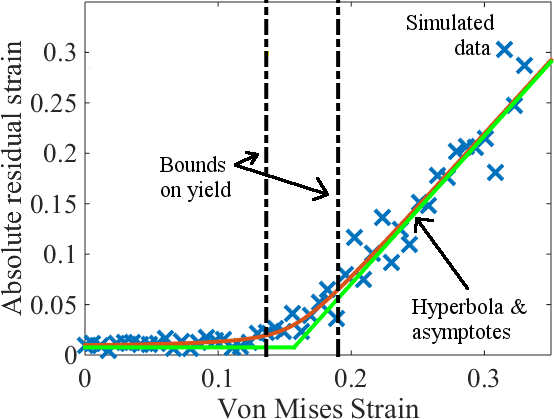
\includegraphics[width=0.9\linewidth]{figures/hyperbola.png}
  \caption{Residual strain $\epsilon_r$ as a function of applied strain $\epsilon$.  Blue $\times$ denote simulated data, whereas the smooth curve is a hyperbola fit to the data.  The green lines are asymptotes; their intersection can be taken as an estimate of $\epsilon_y$.    Bounds on yield are computed by the synthetic data method discussed in Sec.~\ref{sec:bootstrap}. {\it From, ``Estimation and uncertainty quantification of yield via strain recovery simulations,'' P.\ Patrone, CAMX 2016 Conference Proceedings.  Reprinted courtesy of the National Institute of Standards and Technology, U.S. Department of Commerce. Not copyrightable in the United States.}}
  \label{fig:yield}
\end{figure}

While extending this approach to other types of simulations invariably depends on the problem at hand, we recognize a few generic principles.  In particular, it is sometimes possible to test the quality of data by fitting it to {\it global} (not piece-wise or local!) functions that exhibit characteristics we desire of the former.  By testing the goodness of this fit, we can assess the extent to which the data captures the entire structure of the fit-function and therefore conforms to expectations.  We note that this task can even be done in the absence of a known fit function, given only more generic properties such as convexity.  See, for example, the discussion in Ref.~\cite{PatroneAIAA}.


\subsection{Tests based on independent simulations and related ideas}

\begin{figure}
  \centering
  \includegraphics[width=0.9\linewidth]{figures/combinedcluster}
  \caption{Combined clustering between two independent trajectories as a measure of convergence. The X axis is the population of a cluster from trajectory 1, while the Y axis is the population of that cluster from trajectory 2. Cluster populations are show after 20, 100, and 800 ns of sampling. The simulations used to generate the data used in this plot are described in Ref.\ \citep{Roe2014}.}
  \label{f:combinedcluster}
\end{figure}

When estimating any statistical property, multiple measurements are required to characterize the underlying model with high confidence. Consider, for example, the probability that an unbiased coin will land heads-up as estimated in terms of the relative fraction coin-flips that give this result.  This fraction approximated in terms of a single flip (measurement) will always yield a grossly incorrect probability, since only one outcome (heads or tails) can ever be represented by this procedure.  However, as more flips (measurements) are made, the relative fraction of outcomes will converge to the correct probability, i.e., the former represents and increasingly good estimate of the latter.

In an analogous way, we often use ``convergence'' in the context of simulations to describe the extent to which an estimator (e.g., an arithmetic mean) approaches some true value (i.e., the corresponding expectation of an observable) with increasing amounts of data.  In many cases, however, the true value is not known {\it a priori}, so that we cannot be sure what value a given estimator should be approaching.  In such cases, it is common to use the overlap of independent estimates and confidence intervals as a proxy for convergence because the associated clustering suggests a shared if unknown mean.  Conversely, lack of such ``convergence'' is a strong indication that sampling is poor.


There are two approaches to obtaining independent measurements. Arguably the best is to have multiple independent simulations, each with different initial conditions. Ideally these conditions should be chosen so as to span the space to be sampled, which provides confidence that simulations are not being trapped in a local minimum. Consider, for example, the task of sampling the $\phi$ and $\psi$ torsions of alanine dipeptide.  To accomplish this, one could initialize these angles in the alpha-helical conformation and then run a second simulation initialized in the polyproline II conformation. It is important to note, however, that the starting conditions only need to be varied enough so that the desired space is sampled. For example, if the goal is to sample protein folding and unfolding, there should be some simulations started from the folded conformation and some from the unfolded, but if it is not important to consider protein folding, initial unfolded conformations may not be needed.

However, the ``many short trajectories'' strategy has a number of limitations that must be also be considered.  First, as a rule one does not know the underlying ensemble in advance (else, we might not need to do the simulation!), which complicates the generation of a diverse set of initial states. When simulating large biomolecules (e.g. proteins or nucleic acids), ``diverse'' initial structures are often constructed using the crystal or NMR structure coupled with randomized placement of surrounding water molecules, ions, etc.  If the true ensemble contains protein states with significant structural variations, it is possible that no number of short simulations would actually capture transitions, particularly if the transitions themselves are slow.  In that case, each individual trajectory must be of significant duration in order to have any meaning relevant to the underlying ensemble. Th minimum duration needed to achieve significance is highly system dependent, and estimating it in advance requires an understanding of the relevant timescales in the system and what properties are to be calculated.  Second, one must equilibrate each new trajectory, which can appreciably increase the computational cost of running many short trajectories, depending on the quality of the initial states.

One can also try to estimate statistical uncertainties directly from a single simulation by dividing it into two or more subsets (``blocks''). However this can at times be problematic because it can be more difficult to tell if the system is biased by shared initial conditions (e.g., trapped in a local energy minimum). Those employing this approach should take extra care to assess their results (see Sec.~\ref{sec:blockavg}).


Autocorrelation analyses applied to trajectory blocks can be used to better understand the extent to which a time series represents an equilibrated system.  In particular, systems at steady state (which includes equilibrium) by definition have statistical properties that are time-invariant.  Thus, correlations between a single observable at different times depend only on the relative spacing (or ``lag'') between the time steps.  That is, the correlation function has the stationarity property
\begin{equation}
 C(x_j,x_{j+\tau}) = \left< \left(x_j - \expval{x} \right) \left(x_{j+\tau} - \expval{x} \right) \right> = C(\tau)
\end{equation}
where $C(\tau)$ is independent of the time step $j$.  With this in mind, one can partition a given time series into continuous blocks, compute the autocorrelation for a collection of lags $\tau$, and compare between blocks.  Estimates of $C(\tau)$ that are independent of the block suggest an equilibrated (or at least a steady-state) system, whereas significant changes in the autocorrelation may indicate an unequilibrated system.  Importantly, this technique can help to distinguish long-timescale trends in apparently equilibrated data.


\subsubsection*{Combined Clustering}

Cluster analysis is a means by which data points are grouped together based on a similarity (or distance) metric. For example, cluster analysis can be used to identify the major conformational substates of a biomolecule from molecular dynamics trajectory data using coordinate RMSD as a distance metric. For an in-depth discussion of cluster analysis as applied to biomolecular simulations data, see Ref.\ \citep{Shao2007}.

One useful technique for evaluating convergence of structure populations is so-called "combined clustering". Briefly, in this method two or more independent trajectories are combined into a single trajectory (or a single trajectory is divided into two or more parts), on which cluster analysis is performed. Clusters represents groupings of configurations for which intra-group similarity is higher than inter-group similarity \citep{Okur2006}.

The resulting clusters are then split according to the trajectory (or part of the trajectory) they originally came from. If simulations are converged then each part will have similar populations for any given cluster. Indications of poor convergence are large deviations in cluster populations, or clusters that show up in one part but not others. Figure \ref{f:combinedcluster} shows results from combined clustering of two independent trajectories as a plot of cluster population fraction from the first trajectory compared to the second. If the two independent trajectories are perfectly converged then all points should fall on the X=Y line. As simulation time increases the cluster populations from the independent trajectories are in better agreement, which indicates the simulations are converging. For another example of performing combined cluster analysis see Ref.\ \citep{Bergonzo2014}.
